%!TEX root = ../dokumentation.tex

\chapter{Docker Compose}
\label{ch:Docker Compose}
Das vorliegende docker-compose.yaml bildet die Grundlage unserer Containerverwaltung. Durch die Containerorchestrierung öffnen wir durch ein einzelnes Kommando sowohl die Anwendung als auch die Datenbank in ihren eigenen Containern.

Hierbei ist das docker-compose.yaml in drei Bereiche eingeteilt, wobei der services-Bereich wieder in zwei Bereiche eingeteilt werden kann.

\begin{wrapfigure}{r}{0\textwidth}
\centering
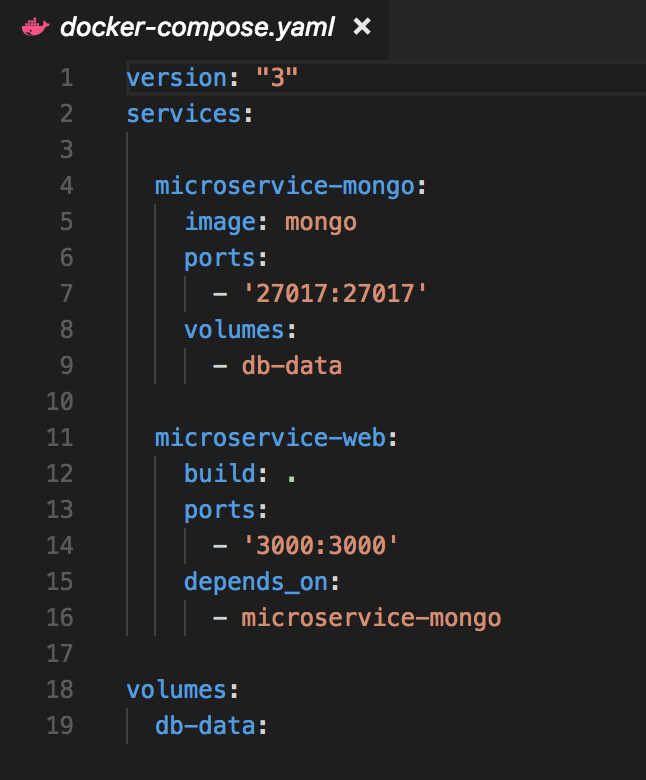
\includegraphics[height=.5\textwidth]{DockerCompose.png}
\vspace{3pt}
\caption{Schaubild\footnotemark}
\label{fig:blueant}
\end{wrapfigure}


Zu aller erst folgt die allgemeinen Angaben zum Compose-File. In unserem Fall besteht diese Information aus der Versionsnummer der Datei.

Der nächste Bereich bildet die unterschiedlichen Services die durch die Orchestrierung aufgebaut werden solllen. Im vorliegenden Fall in die beiden Services \glqq  microservice-mongo\grqq{} und \glqq  microservice-web\grqq{}. Diese stellen unsere beiden Container dar. 
Für den Mongo-DB-Container wird zuerst das Containerimage festgelegt. Dieses wird später von der Imageregistry gezogen und automatisch zu einem Container aufgebaut. Weiter werden die virtuellen Ports auf die lokalen Ports gemappt. Zum Abschluss legt der volumes-Eintrag fest unter welchem Bereich die gesicherten Daten abgelegt werden sollen. Somit lassen sich Container auch entfernen ohne dass die Datensätze verloren gehen.
Für den Anwendungs-Web-Container wird zuerst das Image der Anwendung erstellt. Dies geschieht durch das Kommando build und die Auswahl des aktuellen Directory, in dem auch die Docker-Compose.yaml liegt, durch den Parameter \glqq  Punkt\grqq{}. Auch hier werden die virtuellen auf die lokalen Ports gemappt. Neu an dieser Stelle ist die Abhängigkeit des Anwendungsontainers vom Datenbankcontainer. Diese wird durch \glqq  depends\_on\grqq{} festgelegt.

Im letzten Bereich des Docker-Compose.yamls wird das Volume, auf welches zuvor in der Beschreibung des \glqq  microservice-mongo\grqq{}-Containers bezug genommen wurde, festgelegt und betitelt.

Somit sind alle Vorraussetzungen erfüllt um per "docker-compose up" Befehl die Anwendung und die Datenbank als Container zu starten.
